\documentclass[border=6pt]{standalone}
\usepackage{amsmath}
\usepackage{tikz}
\usetikzlibrary{arrows.meta, positioning, calc, decorations.pathreplacing}

\begin{document}
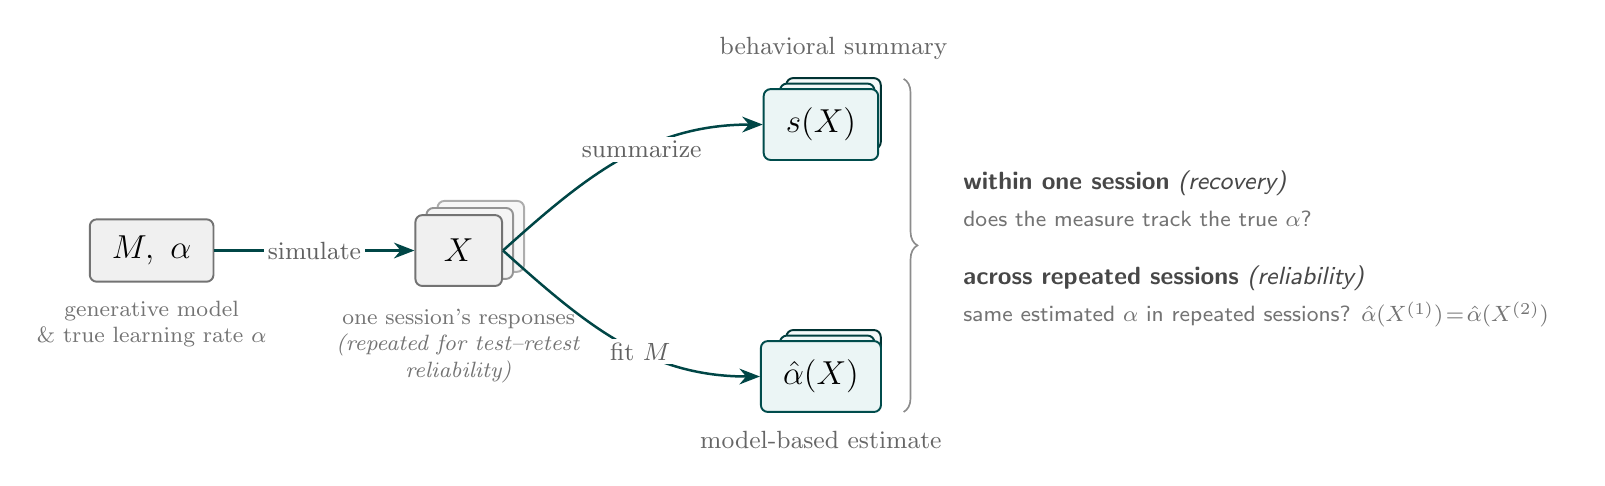
\begin{tikzpicture}[
  font=\sffamily,
  box/.style={draw=teal!60!black, fill=teal!8, rounded corners=2.5pt,
              line width=0.7pt, align=center, inner xsep=8pt, inner ysep=6pt, font=\large},
  truth/.style={box, fill=gray!12, draw=black!55},
  lbl/.style={text=black!60, font=\small, align=center},
  elbl/.style={text=black!62, font=\small, fill=white, inner sep=1.5pt, align=center},
  slbl/.style={text=black!55, font=\footnotesize, align=center},
  ar/.style={-{Stealth[length=2.6mm,width=2mm]}, line width=0.9pt, teal!55!black},
]
% ---- generative model (the known truth) ----
\node[truth] (gen) at (0,0) {$M,\ \alpha$};
\node[slbl, below=3pt of gen] {generative model\\\& true learning rate $\alpha$};

% ---- one session, repeatable (stack = repeated sessions) ----
\node[truth, minimum width=11mm, minimum height=9mm, fill=gray!6, draw=black!32] at (4.18,0.18) {};
\node[truth, minimum width=11mm, minimum height=9mm, fill=gray!9, draw=black!42] at (4.04,0.09) {};
\node[truth, minimum width=11mm, minimum height=9mm] (data) at (3.9,0) {$X$};
\node[slbl, below=4.5pt of data] {one session's responses\\\emph{(repeated for test--retest}\\\emph{reliability)}};
\draw[ar] (gen.east) -- node[elbl]{simulate} (data.west);

% ---- two routes, each a stack: one measure per repeated session ----
\node[box, minimum width=12mm, minimum height=9mm, fill=teal!4, draw=teal!40!black] (summ2) at (8.66,1.74) {};
\node[box, minimum width=12mm, minimum height=9mm, fill=teal!6, draw=teal!50!black] at (8.58,1.67) {};
\node[box, minimum width=12mm, minimum height=9mm] (summ) at (8.5,1.6) {$s(X)$};
\node[lbl, above=3pt of summ2] {behavioral summary};

\node[box, minimum width=12mm, minimum height=9mm, fill=teal!4, draw=teal!40!black] (est2) at (8.66,-1.46) {};
\node[box, minimum width=12mm, minimum height=9mm, fill=teal!6, draw=teal!50!black] at (8.58,-1.53) {};
\node[box, minimum width=12mm, minimum height=9mm] (est) at (8.5,-1.6) {$\hat{\alpha}(X)$};
\node[lbl, below=3pt of est] {model-based estimate};

\draw[ar] (data.east) to[out=42,in=180] node[pos=0.58,elbl]{summarize} (summ.west);
\draw[ar] (data.east) to[out=-42,in=180] node[pos=0.58,elbl]{fit $M$} (est.west);

% ---- evaluation at two scopes ----
\draw[decorate, decoration={brace, amplitude=5pt}, line width=0.6pt, black!45]
   (9.55,2.18) -- (9.55,-2.05);
\node[anchor=west, align=left, text=black!72, inner xsep=10pt] at (9.95,0.02) {%
  \small\textbf{within one session} \emph{(recovery)}\\[1.5pt]
  {\footnotesize\color{black!55} does the measure track the true $\alpha$?}\\[9pt]
  \small\textbf{across repeated sessions} \emph{(reliability)}\\[1.5pt]
  {\footnotesize\color{black!55} same estimated $\alpha$ in repeated sessions? $\hat\alpha(X^{(1)})\!=\!\hat\alpha(X^{(2)})$}};
\end{tikzpicture}
\end{document}
